\documentclass{ximera}

%% You can put user macros here
%% However, you cannot make new environments

\listfiles

\graphicspath{{./}{firstExample/}{secondExample/}}

\usepackage{tikz}
\usepackage{tkz-euclide}
\usepackage{tikz-3dplot}
\usepackage{tikz-cd}
\usetikzlibrary{shapes.geometric}
\usetikzlibrary{arrows}
\usetikzlibrary{decorations.pathmorphing,patterns}
\usetkzobj{all}
\pgfplotsset{compat=1.13} % prevents compile error.

\renewcommand{\vec}[1]{\mathbf{#1}}
\newcommand{\RR}{\mathbb{R}}
\newcommand{\dfn}{\textit}
\newcommand{\dotp}{\cdot}
\newcommand{\id}{\text{id}}
\newcommand\norm[1]{\left\lVert#1\right\rVert}
 
\newtheorem{general}{Generalization}
\newtheorem{initprob}{Exploration Problem}

\tikzstyle geometryDiagrams=[ultra thick,color=blue!50!black]

\usepackage{mathtools}

\title{Newton's Law of Cooling}


\begin{document}

\begin{abstract}

\end{abstract}

\maketitle



\section*{Newton's Law of Cooling}

Newton's law of cooling states that if an object with temperature
$T(t)$ at time $t$ is in a medium with temperature $T_m(t)$,  the
rate of change of $T$ at time $t$ is proportional to $T(t)-T_m(t)$;
thus,
$T$ satisfies a differential equation of the form
\begin{equation} \label{eq:4.2.1}
T'=-k(T-T_m).
\end{equation}
 Here $k > 0$, since the temperature of the object must decrease if
$T > T_m$, or increase if $T < T_m$.  We'll call $k$  the \textit{temperature decay constant of the medium}.

For simplicity, in this section we'll assume  that the medium is
maintained at a constant temperature $T_m$. This is another example of
 building a simple mathematical model for a physical
phenomenon. Like most mathematical models it has its limitations. For
example, it's reasonable to assume that the temperature of a room
remains approximately constant if the cooling object is a cup of
coffee, but perhaps not if it's a huge cauldron of molten metal. 


To solve  \eqref{eq:4.2.1}, we rewrite it as
$$
T'+kT=kT_m.
$$
Since $e^{-kt}$ is a solution of the complementary equation, the
solutions of this equation are of the form $T=ue^{-kt}$, where
$u'e^{-kt}=kT_m$, so $u'=kT_me^{kt}$. Hence,
$$
u=T_me^{kt}+c,
$$
so
$$
T=ue^{-kt}=T_m+ce^{-kt}.
$$
If $T(0)=T_0$,  setting $t=0$ here yields $c=T_0-T_m$, so
\begin{equation} \label{eq:4.2.2}
T=T_m+(T_0-T_m)e^{-kt}.
\end{equation}
Note that $T-T_m$ decays exponentially, with decay constant $k$.


\begin{example}\label{example:4.2.1}
A ceramic insulator is baked at $400^\circ$C and cooled in a room in
which the temperature is $25^\circ$C. After 4 minutes the
temperature of the insulator is $200^\circ$C. What is its temperature
after 8 minutes?
\begin{explanation} Here $T_0=400$ and $T_m=25$, so \eqref{eq:4.2.2} becomes
\begin{equation} \label{eq:4.2.3}
T=25+375e^{-kt}.
\end{equation}
 We determine $k$ from the stated condition that  $T(4)=200$;
that is,
$$
200=25+375e^{-4k};
$$
 hence,
$$
e^{-4k} = \frac{175}{375} = \frac{7}{15}.
$$
 Taking logarithms and solving for $k$ yields
$$
k=-\frac{1}{4} \ln \frac{7}{15}=\frac{1}{4}\ln \frac{15}{7}.
$$
 Substituting this into \eqref{eq:4.2.3} yields
$$
T=25+375 e^{-\frac{t}{4} \ln \frac{15}{7}}
$$
%(Figure~\ref{figure:4.2.1}).
Therefore the temperature of the insulator after
8 minutes is
$$\begin{array}{rl}
T(8) & = 25+375 e^{-2 \ln \frac{15}{7}} \\
& = 25+375 \left(\frac{7}{15}\right)^2 \approx
107^\circ \mbox{C}.
\end{array}$$

\begin{image}
  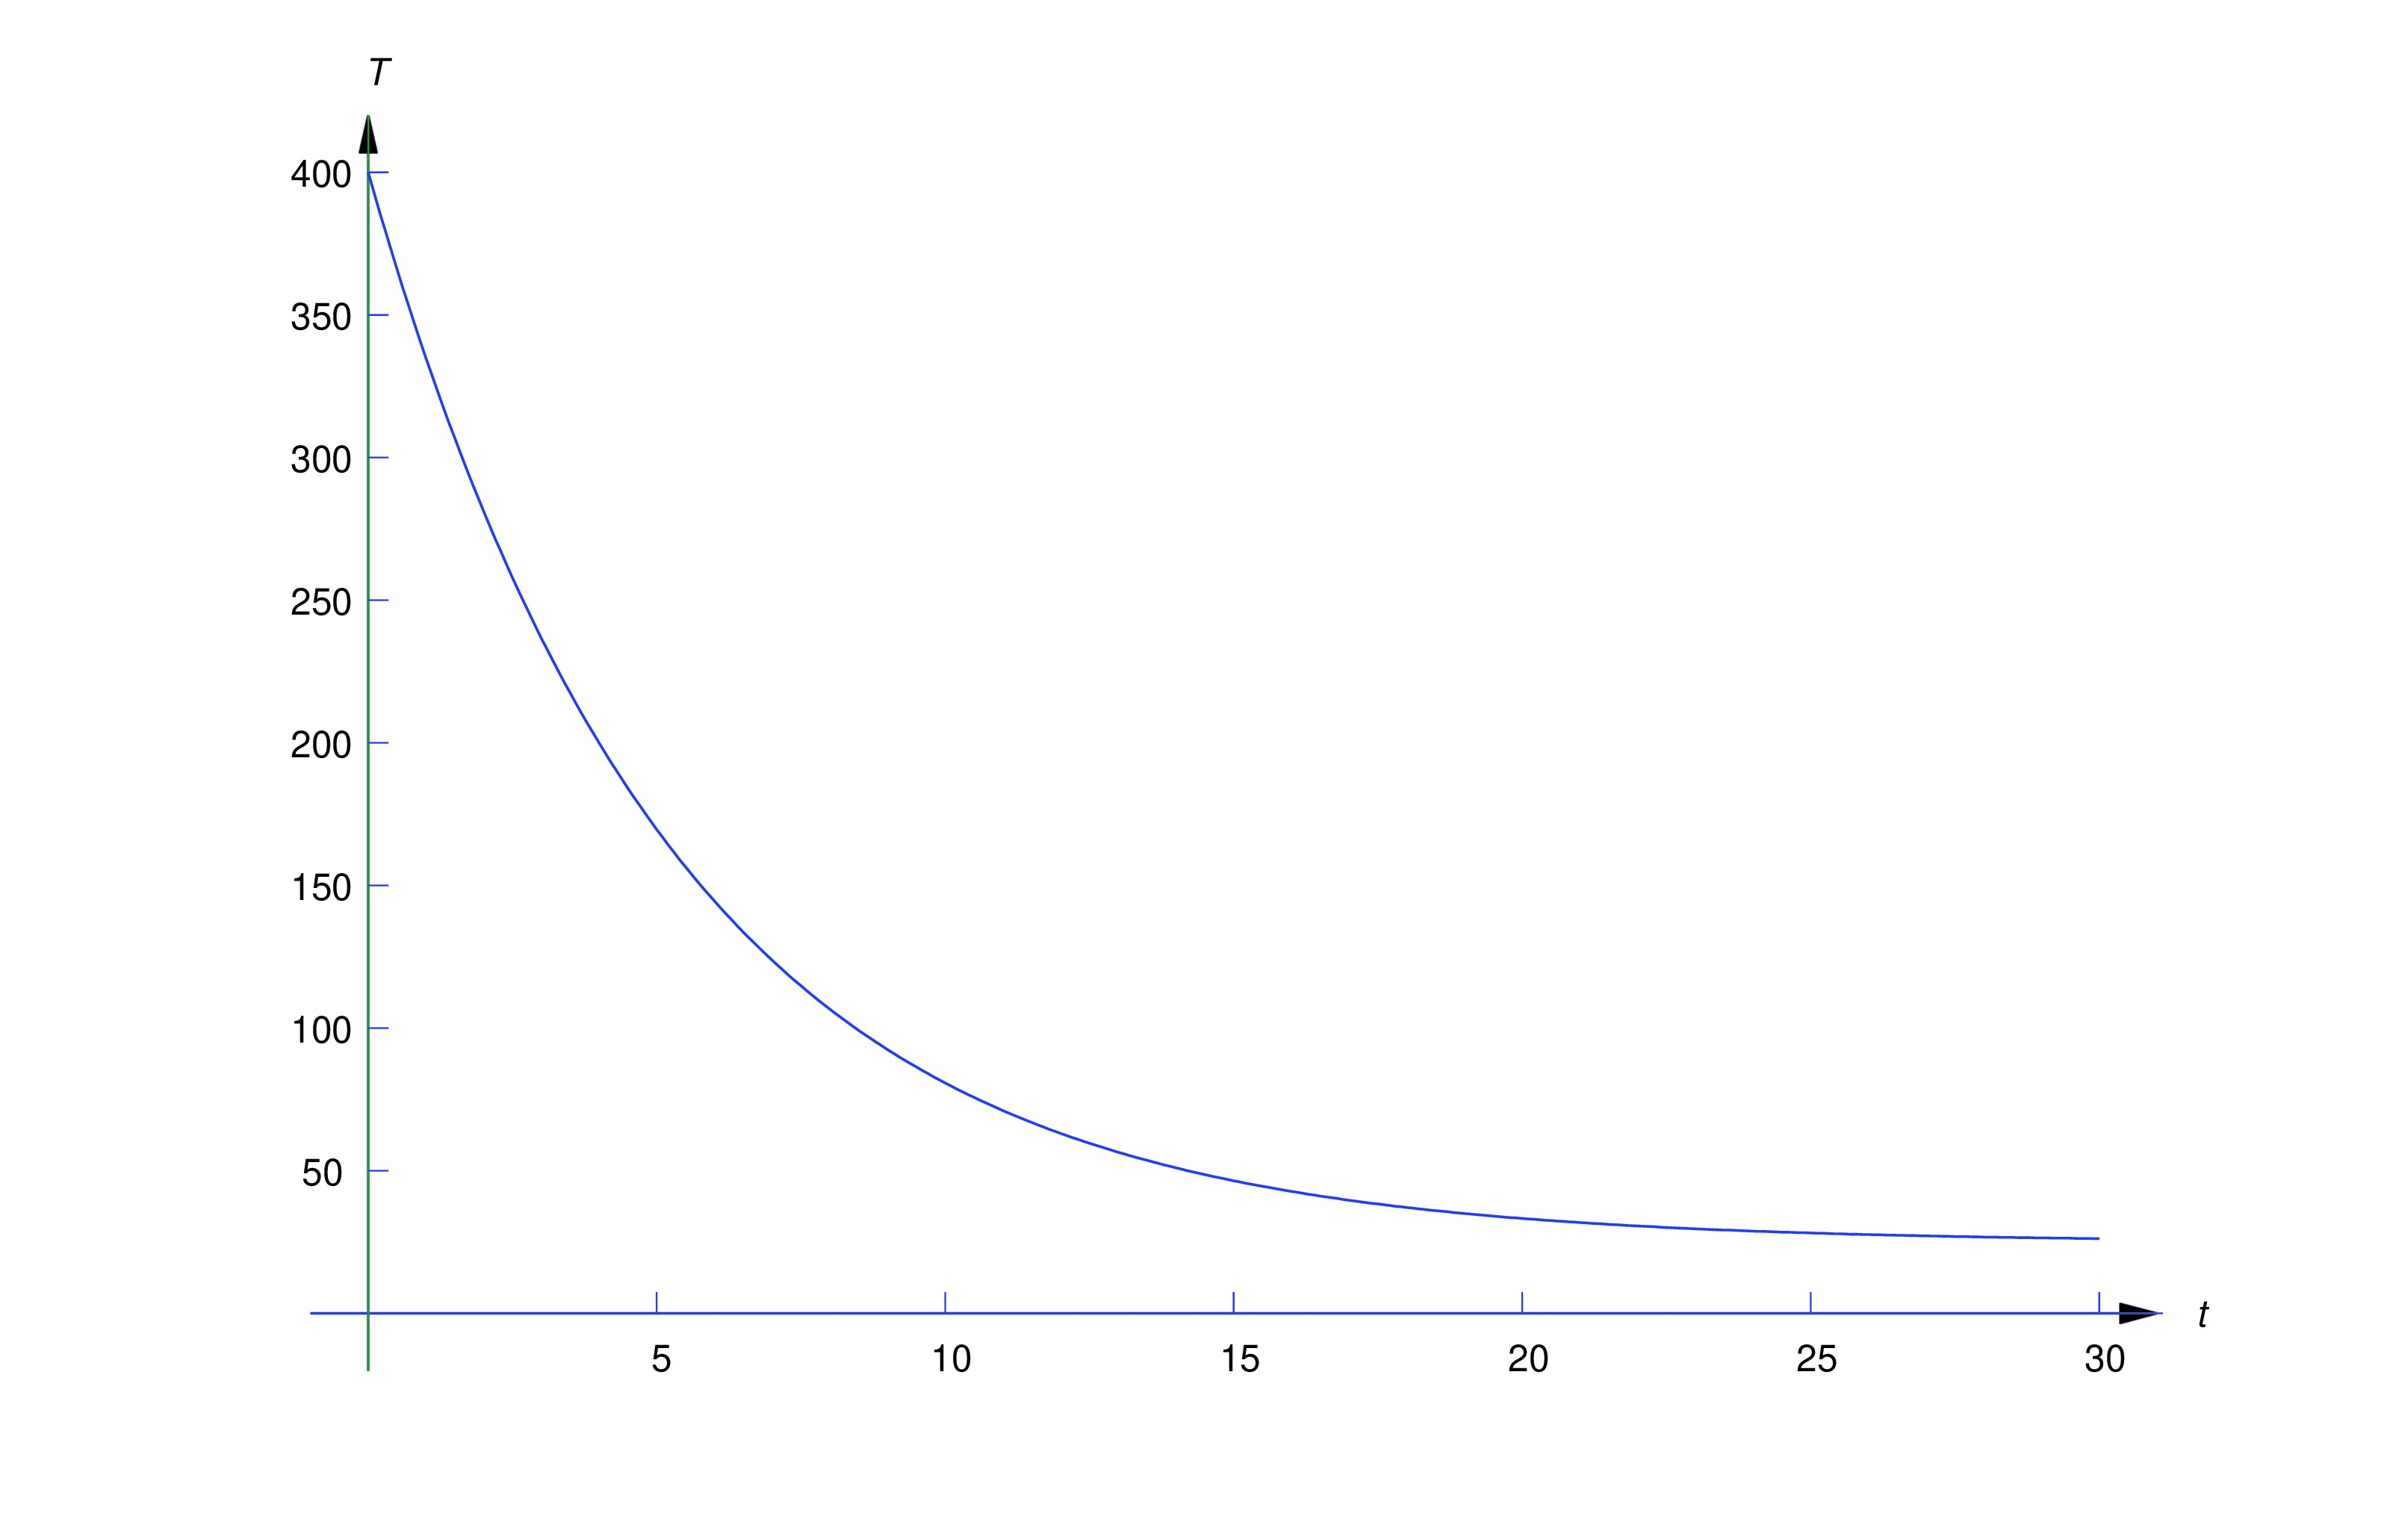
\includegraphics[height=1.5in]{fig040201.jpg} \end{image}
\end{explanation}
\end{example}

\begin{example}\label{example:4.2.2}
An object with temperature $72^\circ$F is placed outside, where the
temperature is $-20^\circ$F. At 11:05 the temperature of the object
is $60^\circ$F and at 11:07 its temperature is $50^\circ$F. At what
time was the object placed outside?


\begin{explanation} Let $T(t)$ be the temperature of the object at time $t$. For
convenience, we choose the origin $t_0=0$ of the time scale to be
11:05 so that $T_0=60$. We must determine the time $\tau$ when
$T(\tau)=72$. Substituting $T_0=60$ and $T_m=-20$ into \eqref{eq:4.2.2}
yields
$$
T  = \answer{-20}+\left(\answer{60}-\answer{-20}\right)e^{-kt}
$$
 or
\begin{equation} \label{eq:4.2.4}
T = \answer{-20}+\answer{80}e^{-kt}.
\end{equation}
We obtain $k$ from the stated condition that the temperature of the
object is $50^\circ$F at 11:07. Since 11:07 is $t=2$ on our time
scale, we can determine $k$ by substituting $T=50$ and $t=2$ into
\eqref{eq:4.2.4} to obtain
$$
50 = -20+80e^{-2k}
$$
 hence,
$$
e^{-2k}=\frac{\answer{7}}{8}.
$$
 Taking logarithms and solving for $k$ yields
$$
k =-\frac{1}{2} \ln \frac{\answer{7}}{\answer{8}} = \frac{1}{2} \ln \frac{\answer{8}}{7}.
$$
\begin{hint}
 Recall that $-\ln (a/b)=\ln (a/b)^{-1}=\ln (b/a)$.
\end{hint}
 Substituting this into \eqref{eq:4.2.4} yields
$$
T = -20+80 e^{-\frac{t}{2}\ln \frac{8}{7}},
$$
 and the condition $T(\tau)=72$  implies that
$$
72 =-20+80 e^{-\frac{\tau}{2} \ln \frac{8}{7}};
$$
 hence,
$$
e^{-\frac{\tau}{2} \ln \frac{8}{7}} =
\frac{\answer{23}}{20}.
$$
Taking logarithms and solving for $\tau$ yields
$$
\tau = -\frac{2 \ln \frac{23}{20}}{\ln \frac{8}{7}} \approx -2.09
\mbox{min}.
$$
Therefore the object was placed outside
about $\answer{2}$ minutes and $\answer{5}$ seconds before 11:05; that is,
at $11:\answer{02}:\answer{55}$.

\begin{image}
  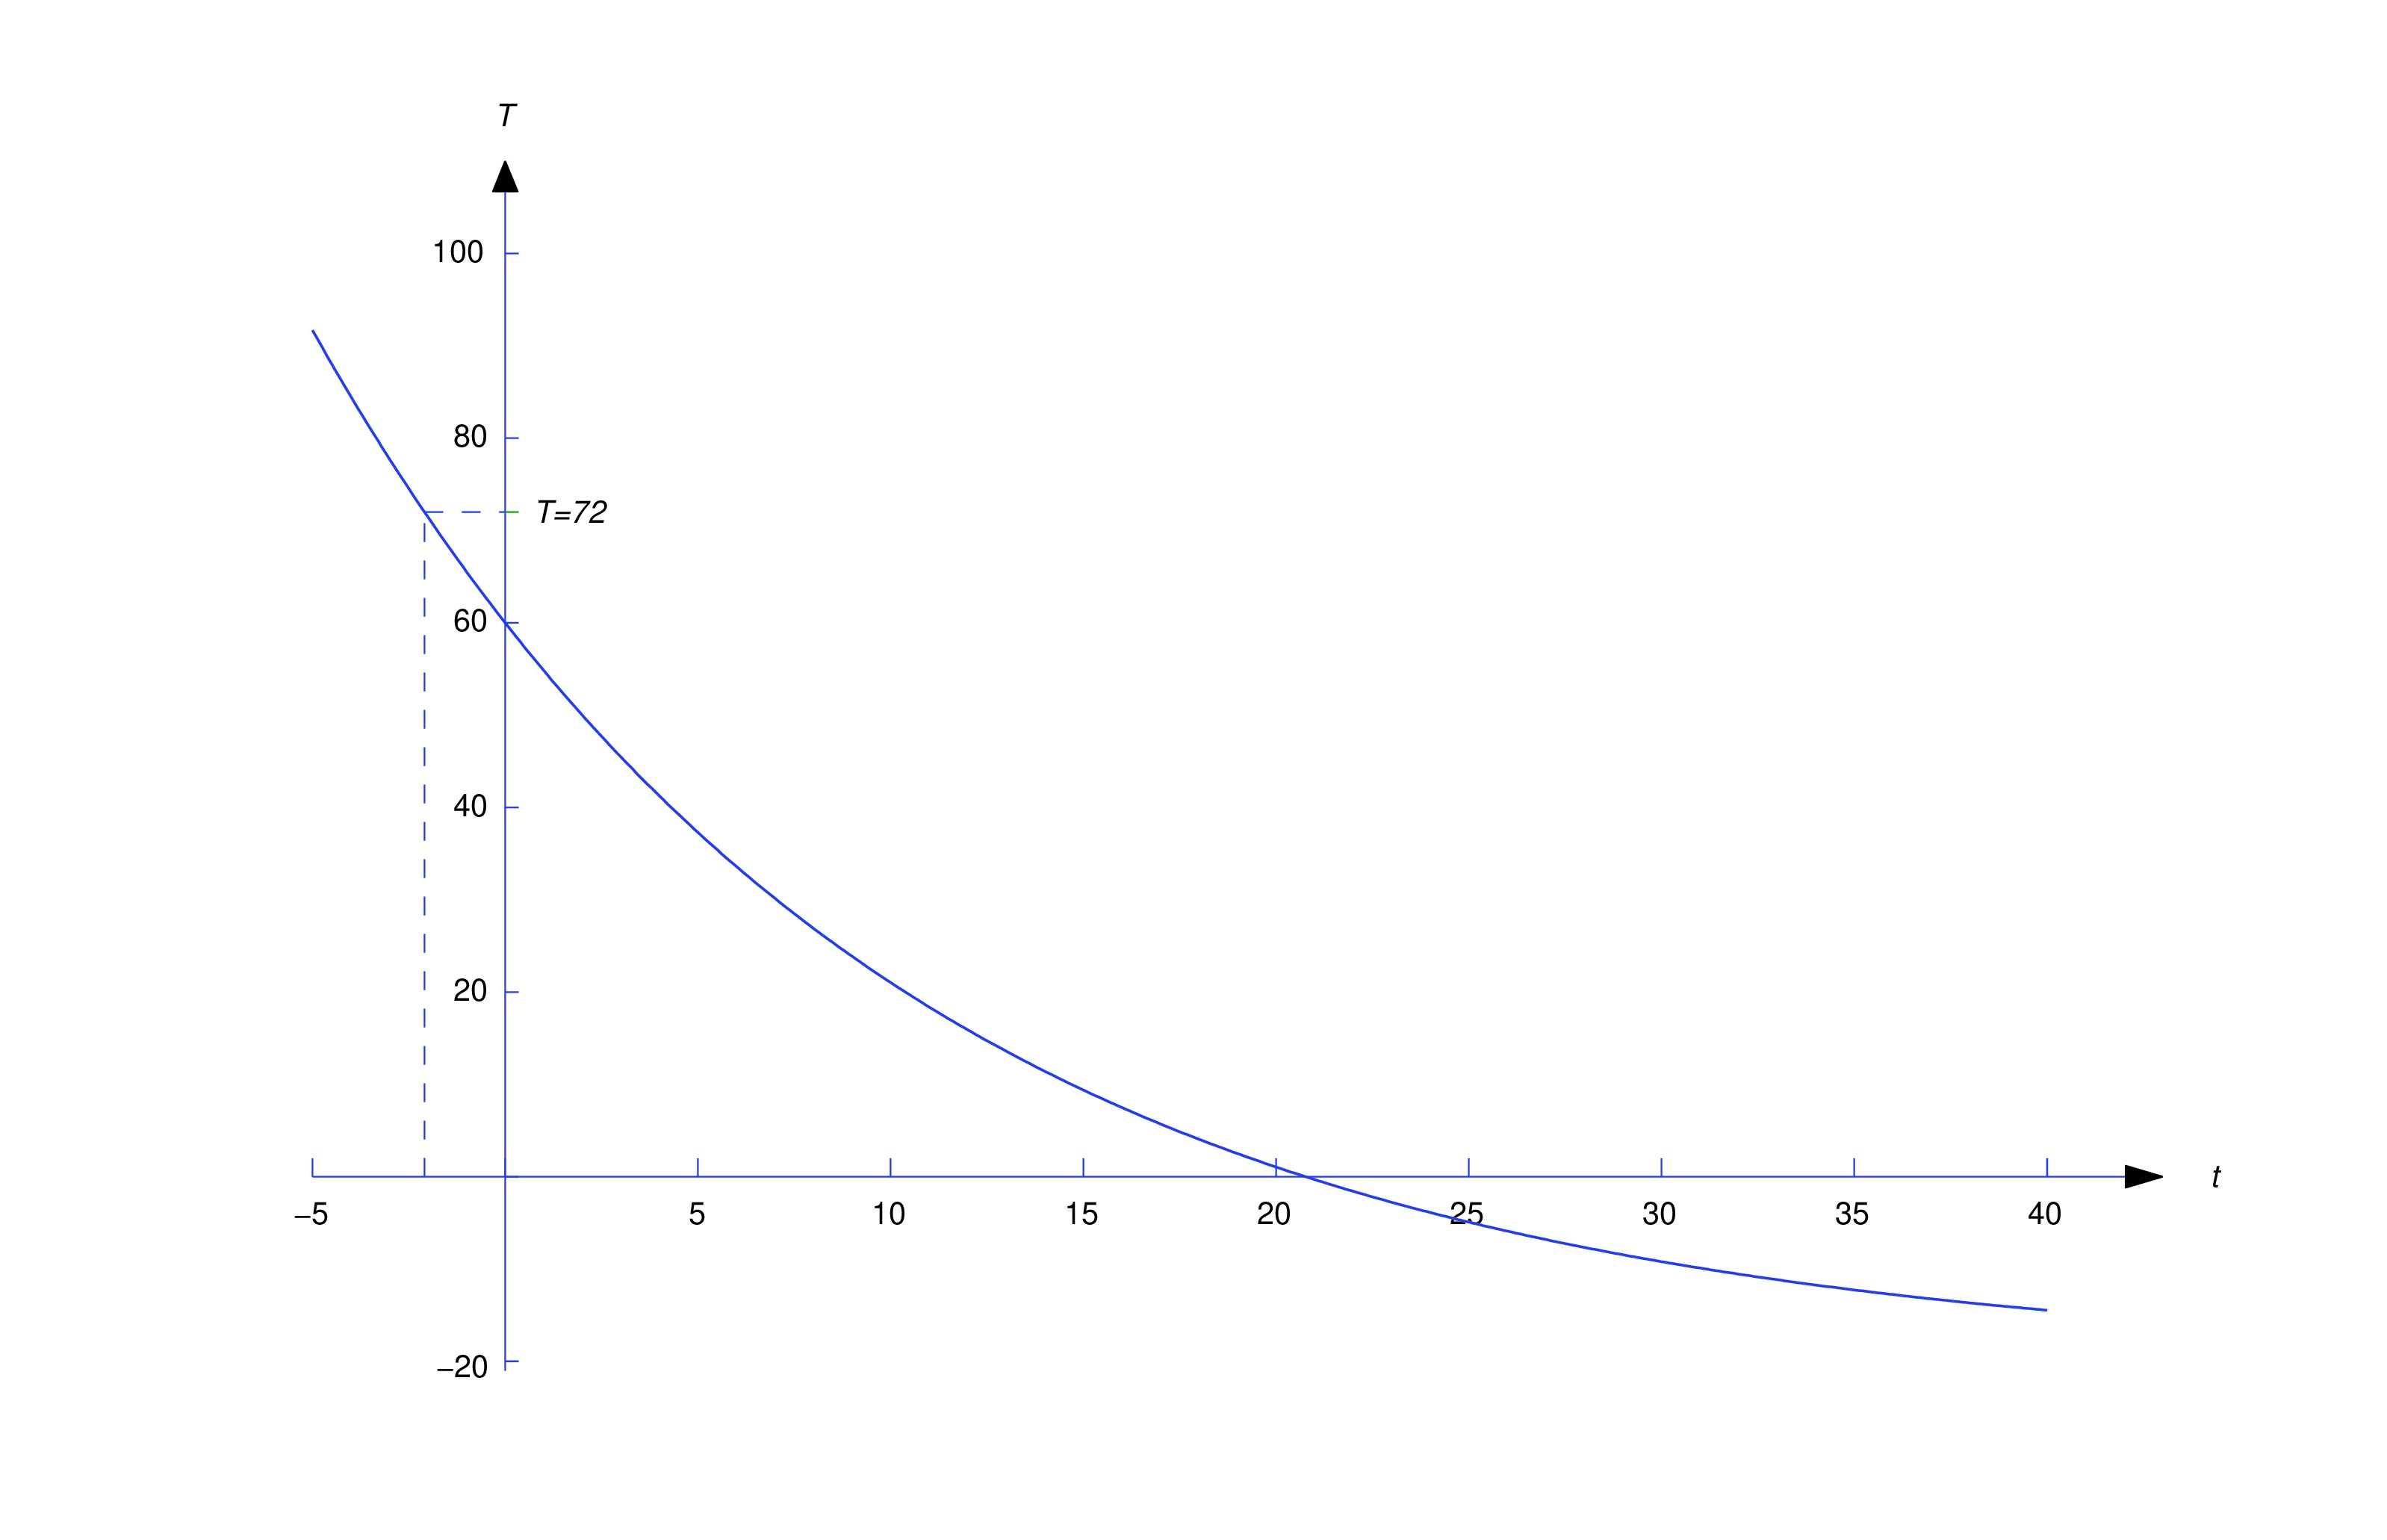
\includegraphics[height=1.5in]{fig040202.jpg} \end{image}

\end{explanation}
\end{example}

\section*{Text Source}
Trench, William F., "Elementary Differential Equations" (2013). Faculty Authored and Edited Books \& CDs. 8. (CC-BY-NC-SA)

\href{https://digitalcommons.trinity.edu/mono/8/}{https://digitalcommons.trinity.edu/mono/8/}


\end{document}